\section{Chapter 5: Magnetic Confinement}

\subsection{Explain the main ideas and principles of magnetic plasma confinement.}
\solutionblock{The main idea of magnetic plasma confinement is to use magnetic fields to confine a plasma. Plasma is charged and will therefore gyrate in an applied magnetic field.}

\subsection{Draw and explain the mechanism of the pinch effect in a plasma with a current flowing inside.}
\solutionblock{
It was discovered that a high current flowing through a conductor will cause the conductor to contract (pinch). 
This is due to the magnetic field generated by the current, which will cause a force on the conductor.
\begin{figure}[H]
    \centering
    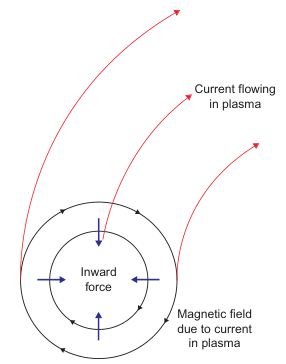
\includegraphics[width=0.5\textwidth]{chapters/fig/5_pinch_effect.png}
    \caption{Pinch effect in a plasma with a current flowing inside.}
    \label{fig:pinch_effect}
\end{figure}
The inward force on the plasma is explained by the Lorentz force acting on the plasma. 
}

\subsection{Draw and explain the gyro-orbits of ions and electrons in a magnetic field. What happens if particles collide?}
\solutionblock{
Charged particles (ions and electrons) will gyrate in a magnetic field. Since the plasma is moving in circular orbits and the magnetic field produced in a Tokamak follows these orbits, the particles will gyrate along their paths. 
\begin{figure}[H]
    \centering
    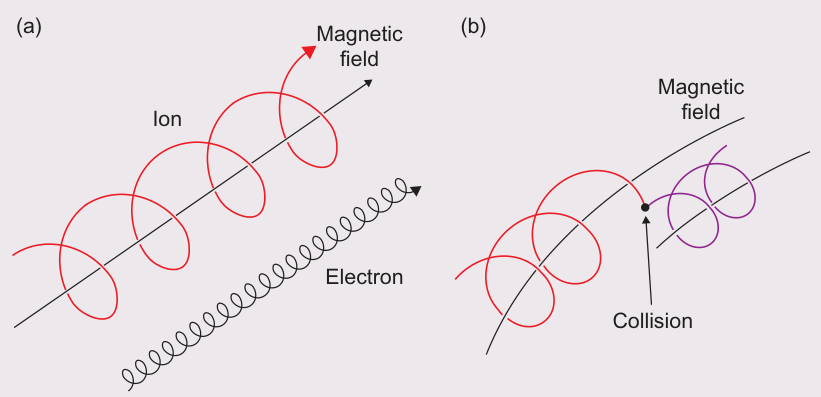
\includegraphics[width=0.5\textwidth]{chapters/fig/5_gyro_orbit.png}
    \caption{Gyro-orbits of ions and electrons in a magnetic field.}
    \label{fig:gyro_orbits}
\end{figure}
Collisions between particles will cause the particles to move to a new orbit. 
}

\subsection{Draw and explain Z-pinch, theta-pinch, and magnetic mirror. How are they related?}
\begin{multisolutionblock}
All three are different ways to confine a plasma using magnetic fields in a linear fashion. 
\begin{figure}[H]
    \centering
    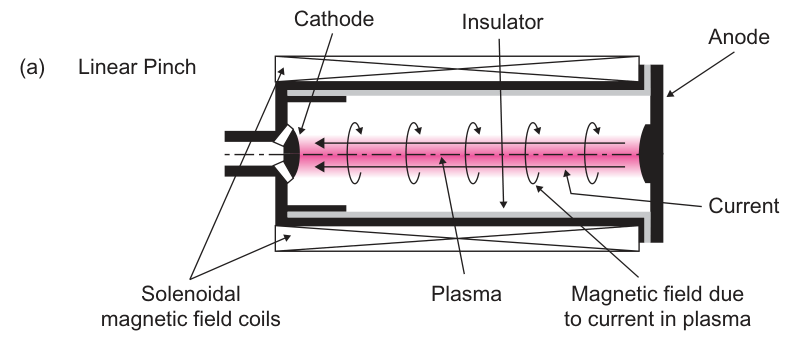
\includegraphics[width=0.5\textwidth]{chapters/fig/5_linear_pinch.png}
    \caption{Z-pinch or linear pinch.}
    \label{fig:z_theta_mirror}
\end{figure}
The Z-pinch uses a current flowing through the plasma to generate a magnetic field that will cause the plasma to contract. It uses an Anode and a Cathode to generate the current in the plasma. 
\begin{figure}[H]
    \centering
    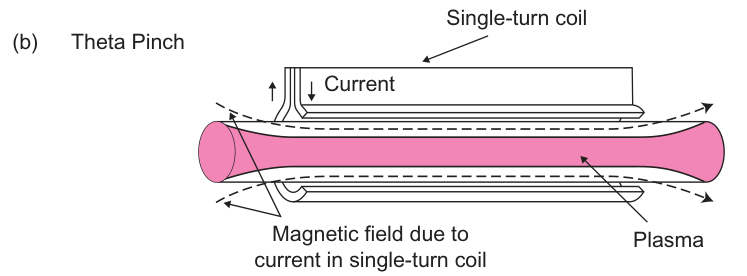
\includegraphics[width=0.5\textwidth]{chapters/fig/5_theta_pinch.png}
    \caption{Theta-pinch.}
    \label{fig:theta-pinch}
\end{figure}
The theta-pinch uses a current flowing through the plasma to generate a magnetic field that will cause the plasma to contract. It uses a current running around the plasma in a single turn coil - along the theta axis in cylindrical coordinates (hence the name). 
\begin{figure}[H]
    \centering
    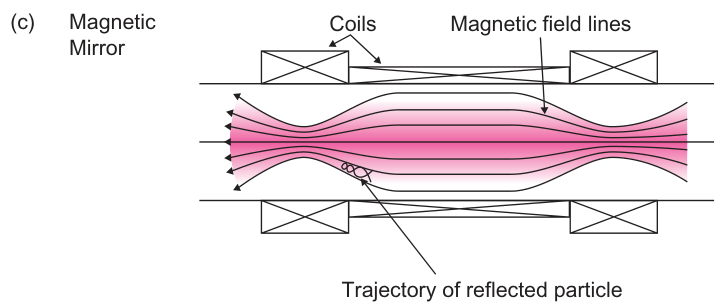
\includegraphics[width=0.5\textwidth]{chapters/fig/5_magnetic_mirror.png}
    \caption{Magnetic mirror.}
    \label{fig:magnetic_mirror}
\end{figure}
Magnetic mirrors use a magnetic field that is stronger at the ends of the plasma than in the middle. This will cause the plasma to be reflected back and forth between the ends of the plasma. Using this method less plasma escapes the magnetic field on each end.
\end{multisolutionblock}

\subsection{What is the plasma beta? Sketch its derivation. How is it related to stability?}
\begin{multisolutionblock}
Plasma beta $\beta$ is the ratio of plasma pressure $p$ to magnetic pressure $p_{mag}$:
\begin{align}
    \beta = \frac{p}{p_{mag}}
\end{align}
Plasma pressure is given by the density $n$ and the temperature $T$ of the plasma: 
\begin{align}
    p = n k_B T
\end{align}
and the magnetic pressure is given by the magnetic field $B$:
\begin{align}
    p_{mag} = \frac{B^2}{2 \mu_0}
\end{align}
Combining these equations gives:
\begin{align}
    \beta = \frac{n k_B T}{B^2 / 2 \mu_0}
\end{align}

$\beta$ is related to stability in the sense that at a higher $\beta$ the plasma is more prone to instabilities. Since for higher plasma pressure the plasma will expand and the magnetic field will be less able to confine the plasma in the device. 
\end{multisolutionblock}

\subsection{Draw and explain instabilities in a Z-pinch. How to avoid them?}
\begin{multisolutionblock}
When an attempt is made to confine the plasma in a Z-pinch, instabilities will occur. Even a small deviation of the magnetic field lines will rapidly lead to a drastic deformation of the plasma.
\begin{figure}[H]
    \centering
    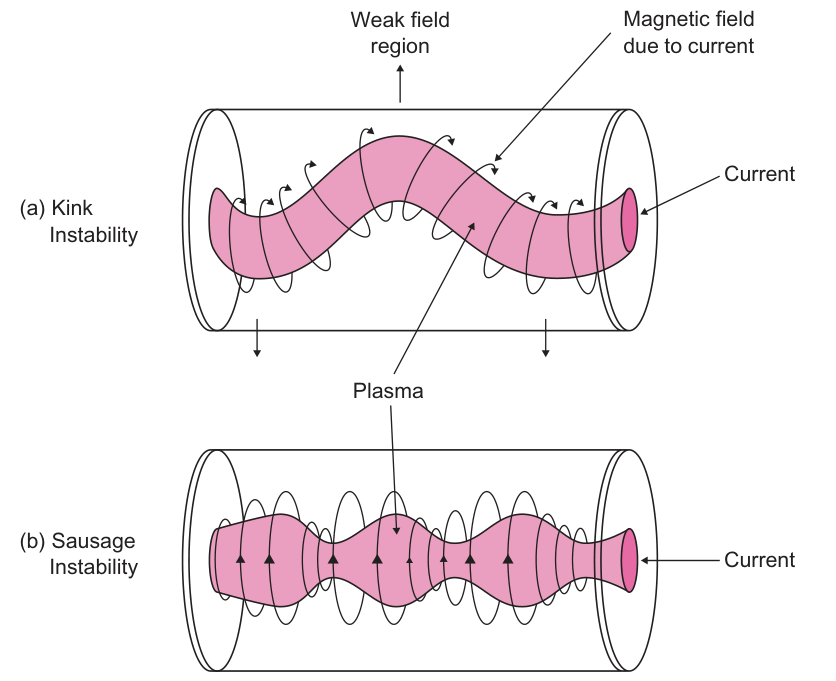
\includegraphics[width=0.5\textwidth]{chapters/fig/5_instabilities.png}
    \caption{Instabilities in Z-pinches.}
    \label{fig:z_pinch_instability}
\end{figure}
To avoid instabilities, the plasma could be confined in a torus. This is the idea behind the Tokamak.
\end{multisolutionblock}

\subsection{Draw and explain a screw pinch and a tokamak. What are similarities and differences?}
\begin{multisolutionblock}
A screw pinch is a combination of a Z-pinch and a theta-pinch much like the grafic bellow: 

\begin{figure}[H]
    \centering
    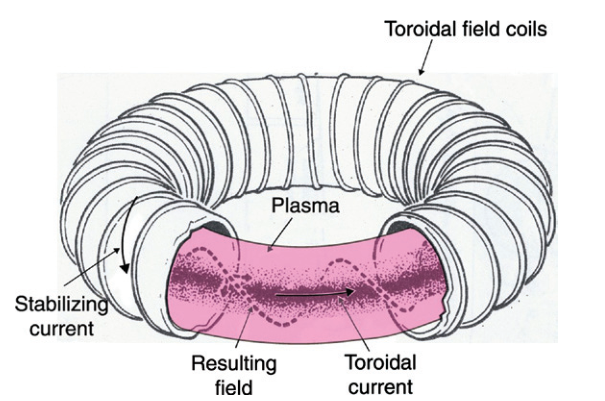
\includegraphics[width=0.5\textwidth]{chapters/fig/5_screw_pinch.png}
    \caption{\textbf{NOTE:} This is a toroidal pinch -> Screw Pinch is linear!!!}
    \label{fig:screw_pinch}
\end{figure}
A Tokamak is a toroidal pinch. It uses a current flowing through the plasma to generate a magnetic field that will cause the plasma to contract. 
\begin{figure}[H]
    \centering
    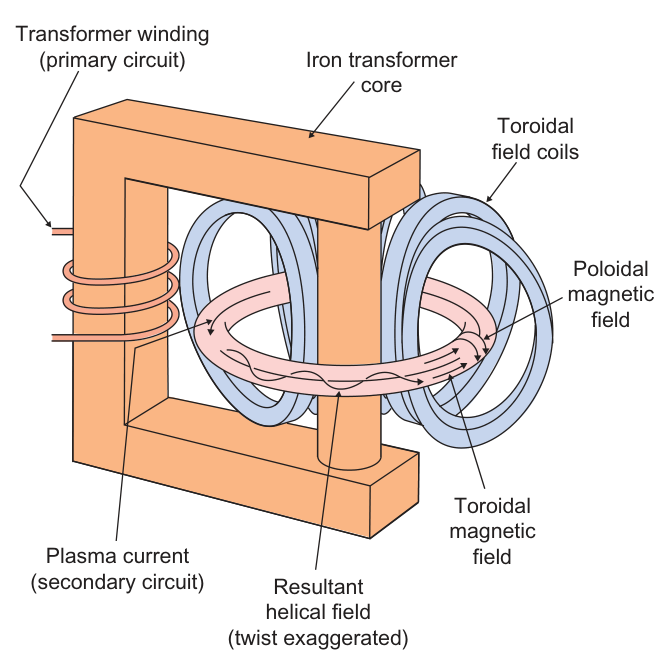
\includegraphics[width=0.5\textwidth]{chapters/fig/5_tokamak.png}
    \caption{Tokamak}
    \label{fig:tokamak}
\end{figure}
\textbf{Similarities:} Both use a current flowing through the plasma to generate a magnetic field that will cause the plasma to contract. \\
\textbf{Differences:} The Tokamak is toroidal and the Screw Pinch is linear. Tokamaks are also more stable than Screw Pinches and don't lose their plasma as easily.
\end{multisolutionblock}

\subsection{Draw and explain a stellarator and explain similarities and differences to a tokamak.}
\solutionblock{
A stellarator is a toroidal device that uses external coils to generate the magnetic field. This means that the current in the plasma is not needed to generate the magnetic field. Compared to a tokamak which is can only be operated in pulsed mode, a stellarator can be operated in steady-state mode.
\begin{figure}[H]
    \centering
    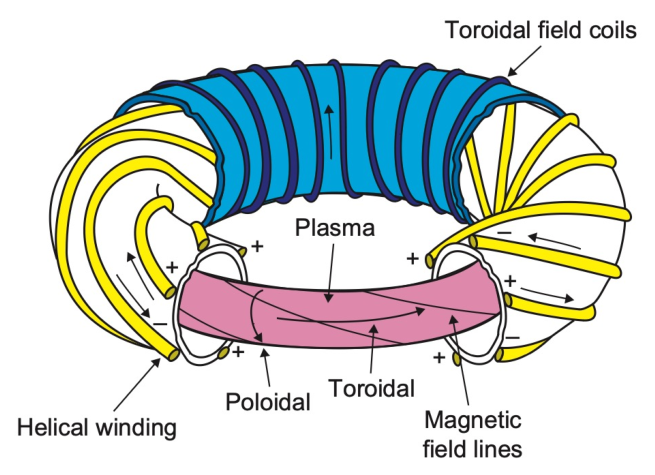
\includegraphics[width=0.5\textwidth]{chapters/fig/5_stellarator.png}
    \caption{Stellarator}
    \label{fig:stellarator}
\end{figure}
\textbf{Similarities:} Both are toroidal devices. \\
\textbf{Differences:} The Tokamak uses a current flowing through the plasma to generate a magnetic field that will cause the plasma to contract. The Stellarator uses external coils to generate the magnetic field.
}
